% DOCUMENTO PRINCIPAL

% Este es el fichero principal de este repositorio. No se recomienda editarlo.
% Modifica las plantillas incluidas en los directorios:
% - secciones
% - tablas
% - algoritmos

\documentclass[final,a4paper,11pt,twoside]{class_diss}

\usepackage[full]{textcomp}
\usepackage{graphicx}
\usepackage{amsmath}
\usepackage{amsxtra}
\usepackage{amssymb}
\usepackage{amsthm}
\usepackage{latexsym}
\usepackage{setspace}
\usepackage[margin=3cm]{geometry}
\usepackage[titles]{tocloft}
\usepackage{latexsym}
\usepackage{fancyhdr}
\usepackage{emptypage}
\usepackage[svgnames,dvipsnames,usenames,table,xcdraw]{xcolor}
\usepackage{tikz}
\usepackage[toc,acronym,nonumberlist,xindy={language=spanish-traditional},sanitize=none]{glossaries}
\usepackage[scaled]{helvet}
\usepackage[utf8]{inputenc}
\usepackage[T1]{fontenc}
\usepackage[spanish,es-tabla]{babel}
\usepackage[explicit]{titlesec}
\usepackage{newtxtext}
\usepackage{newtxmath}
\usepackage{stmaryrd}
\usepackage{bbold}
\usepackage[ruled,vlined]{algorithm2e}
\usepackage{algorithmic}
\usepackage{float}
\usepackage{url}
\usepackage{xspace}
\usepackage{booktabs}
\usepackage{multirow}
\usepackage{enumitem}
\usepackage{rotating}
\usepackage{pdflscape}
\usepackage{listings}
\usepackage{placeins}
\usepackage{flafter}

\theoremstyle{definition}
\newtheorem{definition}{Teorema}[section]
\theoremstyle{remark}
\newtheorem*{remark}{Remark}
\DeclareMathOperator*{\argmax}{arg\,max}
\DeclareMathOperator*{\argmin}{arg\,min}
\definecolor{VIU}{RGB}{240, 90, 15}
\definecolor{DESTACADO}{RGB}{130, 34, 145}
\definecolor{CITA}{RGB}{0, 123, 194}

\renewcommand{\algorithmcfname}{Algoritmo}
\renewcommand{\acronymname}{Lista de Acr\'onimos}
\addto\captionsspanish{
    \renewcommand*{\acronymname}{Lista de Acr\'onimos}
}
\newcommand{\inhib}{\relbar\mapsfromchar}
\newcommand{\destacado}[1]{\color{DESTACADO}\textbf{#1}\color{black}\xspace}

\usetikzlibrary{shapes}
\newcommand*\circled[1]{\tikz[baseline=(char.base)]{
    \node[shape=diamond,fill=black!90,inner sep=1pt,minimum size=1cm] (char) {\textcolor{white}{\small\textbf{#1}}};}
}

\pagestyle{fancy}
\fancyhf{}
\fancyhead[LO]{}
\fancyhead[RE]{}
\fancyfoot[C]{}
\renewcommand{\headrulewidth}{0pt}

\fancypagestyle{plain}{
  \fancyhf{}
  \fancyfoot[C]{\circled{\thepage}}
  \renewcommand{\headrulewidth}{0pt}
}

\colorlet{chapnumcolor}{VIU}

\newcommand*{\chapnumfont}{%
  \usefont{T1}{jkp}{b}{n}%
  \fontsize{70}{90}%
  \selectfont%
}

\newcommand*{\chaptitlefont}{%
  \usefont{T1}{qhv}{b}{n}%
  \fontsize{22}{26}%
  \selectfont%
}

\titleformat{name=\chapter}
{\normalfont\huge\bfseries}
{\rlap{\parbox{\textwidth}{\filleft\chapnumfont\color{chapnumcolor}\thechapter}}}
{0pt}
{\rlap{\parbox{0.7\textwidth}{\filright\chaptitlefont #1}}}

\makeglossaries
% GLOSARIO

% Si quieres incluir un glosario y una lista de abreviaturas en tu Trabajo Fin de Máster,
% sigue las instrucciones indicadas en la siguiente URL:
% https://www.overleaf.com/learn/latex/glossaries

\newacronym{gan}{GAN}{Red Generativa Antagónica o \textit{Generative Adversarial Network}}


\bibliographystyle{apa}

\usepackage[authoryear,sort&compress]{natbib}
\usepackage{hypernat}
\setcitestyle{authoryear}

\usepackage[pdftex,plainpages=false,pdfpagelabels]{hyperref}

\hypersetup{
    linktocpage=true,
    colorlinks=true,
    bookmarks=true,
    citecolor=CITA,
    urlcolor=CITA,
    linkcolor=CITA,
    citebordercolor={1 0 0},
    urlbordercolor={1 0 0},
    linkbordercolor={.7 .8 .8},
    breaklinks=true,
    pdfpagelabels=true,
    }

\setcounter{secnumdepth}{3}
\onehalfspacing
\renewcommand\familydefault{\sfdefault}

\begin{document}

%%%% Incluye la portada oficial%%%%
%% Archivo portada.docx
\cleardoublepage

% Escribe aquí tu frase favorita
\null\vspace{\stretch{2}}
{
\hfill \begin{minipage}{8cm}
\textsl{
\begin{flushright}
    Escribe aquí \\ tu frase favorita.
\end{flushright}
}

% E indica aquí su autor
\begin{flushright}
E indica aquí su autor
\end{flushright}

\end{minipage}
}
\vspace{\stretch{1}}


\pagenumbering{gobble}
% AGRADECIMIENTOS

\cleardoublepage

\normalfont{\huge{\bfseries{Agradecimientos}}}
\vspace{15ex}

% Escribe tus agradecimientos a continuación.
% Se recomienda separar cada párrafo con un \medskip.

Me gustaría agradecer...
\medskip

También quiero destacar...
\medskip

Por último...

\cleardoublepage

\newpage
\pagenumbering{roman}
\setcounter{page}{1}

\pagestyle{fancy}
\fancyhf{}
\fancyhead[LO]{\leftmark}
\fancyhead[RE]{\rightmark}
\fancyfoot[C]{\circled{\thepage}}
\renewcommand{\headrulewidth}{0.4pt}

\pdfbookmark[0]{\contentsname}{contents}

\renewcommand{\cftchapleader}{\cftdotfill{\cftdotsep}}
\renewcommand{\cftchapfont}{\mdseries}
\renewcommand{\cftchappagefont}{\mdseries}

\tableofcontents
\listoffigures
\listoftables

\renewcommand{\listalgorithmcfname}{Índice de algoritmos}
\listofalgorithms
\addcontentsline{toc}{chapter}{Índice de algoritmos}

\newpage
\pagenumbering{arabic}
\setcounter{page}{1}

\cleardoublepage

\chapter*{Resumen}
\label{resumen}
\addcontentsline{toc}{chapter}{Resumen}

% Escribe aquí 

% INTRODUCCIÓN

\cleardoublepage

\chapter{Introducción}
\label{introduccion}

Escribe aquí la introducción de tu Trabajo Fin de Máster, utilizando tantas secciones, subsecciones y subsubsecciones como estimes necesarias.

\section{Mi primera sección}
\label{mi-primera-seccion}

\textbf{Esta palabra} está en negrita. \textit{Esta palabra} está en cursiva. \destacado{Esta palabra} se destaca en púrpura.
\medskip

\section{Mi segunda sección}
\label{mi-segunda-seccion}

En la sección~\ref{mi-primera-seccion} se muestran ejemplos de palabras en negrita, cursiva y destacadas en púrpura.
\medskip

% Define los acrónimos en el fichero secciones/glosario.tex
% Define la bibliografía en el fichero bibliografia.bib
Una \acrfull{gan} es... \citep{goodfellow2014generative}.
\medskip

\citet{goodfellow2014generative} diseñaron las redes generativas antagónicas como...
\medskip

\vspace{5ex}

Listado:
\begin{itemize}
  \item Item 1.
  \item Item 2.
  \item Item 3.
\end{itemize}

Enumeración:
\begin{enumerate}
  \item Item 1.
  \item Item 2.
  \item Item 3.
\end{enumerate}

\subsection{Una subsección}
\label{una-subseccion}

La figura~\ref{fig1} muestra...

\begin{figure}[ht!]
    \centering
    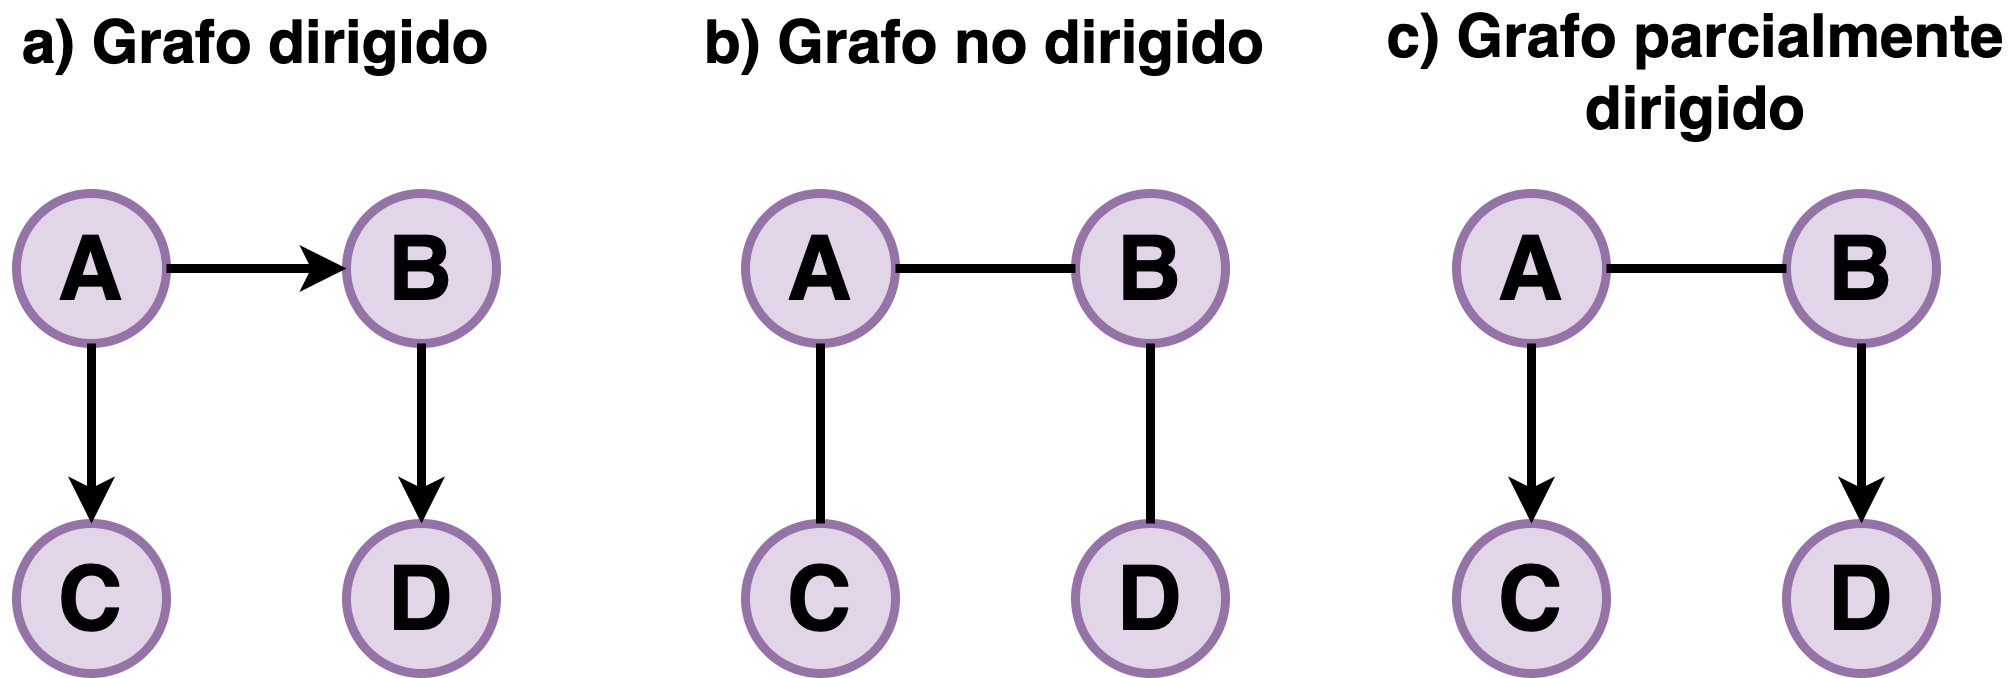
\includegraphics[scale=0.15]{figuras/fig1.png}
    % \caption[Así aparece el rótulo en el índice]{Así aparece el rótulo en el texto.}
    \caption[Tipos de grafos]{\textbf{Tipos de grafos.}}
    \label{fig1}
\end{figure}

La tabla~\ref{tab1} muestra...

\begin{table}[ht!]
\centering
\resizebox{\textwidth}{!}{
\begin{tabular}{@{}ccccc@{}}
\toprule
\textbf{Columna 1} & \textbf{Columna 2} & \textbf{Columna 3} & \textbf{Columna 4} & \textbf{Columna 5} \\ \midrule
Fila 1             & A                  & B                  & C                  & D                  \\ \midrule
Fila 2             & E                  & F                  & G                  & H                  \\ \midrule
Fila 3             & I                  & J                  & K                  & L                  \\ \bottomrule
\end{tabular}
}
% \caption[Así aparece el rótulo en el índice]{Así aparece el rótulo en el texto.}
\caption[Ejemplo de tabla]{\textbf{Ejemplo de tabla.}}
\label{tab1}
\end{table}


\subsection{Una subsubsección}
\label{una-subsubseccion}

El algoritmo~\ref{alg1} muestra...
\medskip

\begin{algorithm}[H]
\label{alg1}
\SetAlgoLined
\medskip
\begin{enumerate}
    \item Elegir una estructura de red $\mathcal{G}$ sobre $\mathbf{V}$, normalmente vacía. Establecer la puntuación máxima inicial: $Score_{max} = Score_{\mathcal{G}}$.
    \item Repetir los siguientes pasos mientras $Score_{max}$ siga aumentando:
    \begin{enumerate}
        \item Calcular las puntuaciones para todas las posibles redes modificadas $\mathcal{G}^{*}$ que se pueden obtener añadiendo, eliminando o reorientando un solo eje de $\mathcal{G}$ sin que se producan ciclos.
        \item Si para alguna de las redes modificadas $\mathcal{G}^{*}$ se cumple que $Score_{G^{*}} > Score_{\mathcal{G}}$, establecer $G = G^{*}$ y $Score_{max} = Score_{G^{*}}$.
    \end{enumerate}
    \item Devolver el DAG $\mathcal{G}$.
\end{enumerate}
 \caption{Algoritmo \textit{Hill-Climbing} (HC)}
\end{algorithm}


\newpage

Ejemplo de fórmula:

\begin{equation*}
    N_{k}(\mathbf{\mu},\mathbf{\Sigma}) = \frac{1}{\sqrt{2\pi\det(\Sigma})} \exp \bigg\{ -\frac{1}{2}(\mathbf{X}-\mathbf{\mu})^{T}\Sigma^{-1}(\mathbf{X}-\mathbf{\mu}) \bigg\} \quad \mathbf{X},\mathbf{\mu} \in \mathbb{R}^{k}
\end{equation*}

Otro ejemplo de fórmula:

\begin{equation*}
    \underbrace{P(\mathcal{B}|\mathcal{D}) = P(\mathcal{\mathcal{G}},\Theta|\mathcal{D})}_{\textbf{Aprendizaje}} = \underbrace{P(\mathcal{G}|\mathcal{D})}_{\textbf{Aprendizaje estructural}} \cdot \underbrace{P(\Theta|\mathcal{G},\mathcal{D})}_{\textbf{Aprendizaje paramétrico}}
\end{equation*}

% OBJETIVOS

\cleardoublepage

\chapter{Objetivos}
\label{objetivos}

Describe aquí el objetivo general de tu Trabajo Fin de Máster y, a continuación, define los objetivos parciales:
\medskip
\begin{enumerate}[label=\destacado{\arabic*.}]
  \setlength\itemsep{1em}
  \item \textbf{Objetivo parcial 1.}

  \item \textbf{Objetivo parcial 2.}

  \item \textbf{Objetivo parcial 3.}
\end{enumerate}

% METODOLOGÍA

\cleardoublepage

\chapter{Metodología}
\label{metodologia}

% RESULTADOS Y DISCUSION 

\cleardoublepage

\chapter{Resultados y Discusión}
\label{resultados-y-discusion}

% CONCLUSIONES

\chapter{Conclusiones}
\label{conclusiones}

\begin{enumerate}[label=\destacado{\arabic*.}]
  \setlength\itemsep{1em}
  \item Conclusión 1.

  \item Conclusión 2.

  \item Conclusión 3.
\end{enumerate}

% LIMITACIONES Y PERSPECTIVAS DE FUTURO

\cleardoublepage

\chapter{Limitaciones y\\ Perspectivas de Futuro}
\label{limitaciones-y-futuro}


\cleardoublepage
\phantomsection

\printglossary[type=\acronymtype]
\printglossary

\appendix
% APÉNDIZES

% Escribe cada apéndize como si fuera un capítulo más.

\chapter{Apéndize A}
\label{apendize-a}

\chapter{Apéndize B}
\label{apendize-b}


\begin{singlespace}
\begin{footnotesize}
\begin{twocolumn}
\bibdata{bibliografia}
\bibliography{bibliografia}
\addcontentsline{toc}{chapter}{Bibliografía}
\end{twocolumn}
\end{footnotesize}
\end{singlespace}

\end{document}
